\documentclass[compress]{beamer}
\mode<presentation>
{
 \usetheme{Vilanova}
}

\usepackage[french]{babel}

\usepackage[utf8]{inputenc}

\usepackage{times}
\usepackage[T1]{fontenc}

\usepackage{amsfonts}
\usepackage{amsmath}
\usepackage{amssymb}
\usepackage{tikz}
\usepackage{eurosym}
%\usepackage{url}
\usepackage[normal]{subfigure}
\newcommand{\goodgap}{%
	\hspace{\subfigtopskip}%
	\hspace{\subfigbottomskip}}



%\newtheorem{definition}{Definition}

\title{Traitement d'images de télédétection}

\subtitle{La main à la pâte avec OTB/Monteverdi} % (optional)


\author
{jordi.inglada@cesbio.cnes.fr}
\normalsize

\institute[Cesbio] % (optional, but mostly needed)
{\textsc{Centre d'Études Spatiales de la Biosphère, Toulouse, France}}

\date{}

\pgfdeclareimage[height=96mm,width=128mm]{background}{fondsClairSansLogo}
\setbeamertemplate{background}{\pgfuseimage{background}}
\pgfdeclareimage[height=0.6cm]{logoIncrust}{logoIncrust}
\pgfdeclareimage[height=0.5cm]{logo_cesbio}{logo_cesbio}
\logo{
\begin{tabular}{lp{0.25\textwidth}lp{0.25\textwidth}r}
\href{http://www.cesbio.ups-tlse.fr/}{\pgfuseimage{logo_cesbio}}
&&\footnotesize{AUF - Marrakech 2011}&&
\href{http://www.orfeo-toolbox.org}{\pgfuseimage{logoIncrust}}\\
\end{tabular}
}


\subject{Orfeo Toolbox}

% Delete this, if you do not want the table of contents to pop up at
% the beginning of each subsection:
\AtBeginSection[]
{
  \begin{frame}<beamer>
    \frametitle{Plan}
%     \tableofcontents[currentsection,currentsubsection]
\vspace*{-0.5cm}
    \tableofcontents[currentsection]
  \end{frame}
}




% If you wish to uncover everything in a step-wise fashion, uncomment
% the following command: 

% \beamerdefaultoverlayspecification{<+->}

\begin{document}

\begin{frame}
  \titlepage
  \begin{center}
{\tiny Ce contenu est dérivé de la formation \href{http://www.orfeo-toolbox.org/packages/PragmaticRemoteSensing-handout.pdf}{``Pragmatic Remote
  Sensing''} dispensée par J. Inglada et E. Christophe en juillet 2010
  dans le cadre du colloque IGARSS. Il est mis à disposition selon les termes de la licence :\\
Creative Commons Paternité – Partage à l’Identique 3.0 non transcrit.} \href{http://creativecommons.org/licenses/by-sa/3.0/}{
\includegraphics[width=0.05\textwidth]{/home/inglada/Dev/GH/IGARSS2010/Tutorial/Slides/Ressources/CC-licence.png}}    
  \end{center}

\end{frame}

\begin{frame}
\frametitle{Objectifs}
\begin{block}{Obstacles au traitement des images}
\begin{itemize}
 \item Lecture des images
 \item Accès au méta-données
 \item Mise en oeuvre d'algorithmes de l'état de l'art
\end{itemize}
\end{block}
$\Rightarrow$ pour être capable \alert{d'extraire un maximum
  d'informations}, nous avons besoin \alert{d'accéder} aux données et
aux algorithmes,\ldots
\end{frame}


\section{Introduction to the Orfeo Toolbox}



\subsection{L'OTB}
\begin{frame}
\frametitle{Qu'est-ce que l'ORFEO Toolbox (OTB)}

\textbf{Dans le cadre du programme ORFEO du CNES}
\begin{alertblock}{Objectif}
Faciliter le développement et la validation d'algorithmes
\end{alertblock}
\begin{block}{}
\begin{itemize}
 \item Bibliothèque C++ : fournir beaucoup d'algorithmes
   (pre-traitements, extraction d'informations) avec une interface commune.
 \item Logiciel libre : liberté d'utiliser, de modifier, de développer
   son propre logiciel et le revendre!
 \item Multi plate-forme : Windows, Linux, Unix, Mac
\end{itemize}
\end{block}
\end{frame}


\subsection{Un peu d'histoire}
\begin{frame}
\frametitle{Un peu d'histoire}
\begin{block}{Le début (2006)}
\scriptsize
\begin{itemize}
 \item Le CNES finance le développement de la bibliothèque.
 \item Orienté vers la THR (Pléiades), mais utilisation sur d'autres
   capteurs aussi.
 \item Environ 1,000,000\euro~ sur les 4 premières années; budget
   équivalent renouvelé.
\end{itemize}
\end{block}
\begin{block}{Vers des applications faciles à utiliser (2008)}
\scriptsize
\begin{itemize}
  \item Les interactions avec les utilisateurs ont montré le besoin
    d'outils pour les non informaticiens.
  \item Quelques applications avec IHM graphique disponibles.
  \item Plusieurs séances de formation (3-5 jours) en France,
    Belgique, Madagascar, UNESCO, Hawaii, ... et Marrakech!
\end{itemize}
\end{block}
\end{frame}


\subsection{Motivations}
\begin{frame}
\frametitle{Motivations}
\begin{overprint}
\onslide<1->{
\begin{block}{L'OTB, un succès?}
\scriptsize
\begin{itemize}
  \item La communauté d'utilisateurs \alert{croit en permanence}
    (développeurs et utilisateurs)
  \item Présentations régulières dans les conférences internationales
    de télédétection
  \item Le CNES continue à soutenir le développement.
  \item L'analyse de la valeur du logiciel est très encourageante
    (cf. \href{http://www.ohloh.net/p/otb}{Ohloh}): \alert{le
    recyclage est puissant!}
\end{itemize}
\end{block}
}
\onslide<2->{
\begin{block}{Pourquoi faire un logiciel à 1 M\euro~et le
    distribuer gratuitement?}
\scriptsize
\begin{itemize}
 \item Le CNES n'est pas un éditeur de logiciels
 \item Un des objectifs est \alert{le soutien de la recherche} : les
   scientifiques ont besoin de comprendre comment ça marche. 
 \item Le CNES fait des satellites et doit s'assurer que \alert{les
   images sont utilisées}
\end{itemize}
\end{block}
}
\end{overprint}
\end{frame}


\subsection[How]{Comment?}
% Using other library
\begin{frame}
\frametitle{Comment?}
\begin{overprint}
\onslide<1->{
\begin{block}{Comment y arriver?}
En utilisant ce qui existe déjà!
\end{block}
}
\onslide<2->{
\begin{block}{Beaucoup de bibliothèques libres de bonne qualité}
\scriptsize
\begin{itemize}
  \item ITK : architecture du logiciel (streaming, multithreading),
    beaucoup d'algorithmes de traitement d'images
 \item Gdal/Ogr: lécture et écriture de différents formats de données (geotiff, raw, png, jpeg, shapefile, \ldots)
 \item Ossim: modèles géométriques de capteur (Spot, RPC, SAR, \ldots)
   et projections cartigraphiques
 \item 6S: corrections radiométriques
 \item et beaucoup d'autres : libLAS (lidar), Edison (clustering Mean Shift), libSiftFast (SIFT), Boost (graphes), libSVM (Support Vector Machines)
\end{itemize}
\normalsize
\alert{$\Rightarrow$ accessibles via une interface commune}
\end{block}
}
\end{overprint}
\end{frame}


\section{Fonctionnalités}

\subsection{Composants}

\begin{frame}
\frametitle{Composants disponibles}
 \begin{block}{}
\scriptsize
\begin{itemize}
\item La plupart de formats d'images
\item Corrections géométriques
\item Corrections rediométriques
\item Détection de channgements
\item Extraction de primitives
\item Classification
\end{itemize}
\end{block}


 \begin{block}{Documentation}
\scriptsize
\begin{itemize}
\item Software Guide (+600 pages pdf), et aussi
  \href{http://www.orfeo-toolbox.org/SoftwareGuide/}{version en ligne}
\item \href{http://www.orfeo-toolbox.org/doxygen}{Doxygen}:
  documentation pour développeurs
\end{itemize}
\end{block}
\end{frame}

\subsection{Architecture}

\begin{frame}
 \frametitle{Une architecture puissante}
  \begin{block}{Modulaire}
\scriptsize
\begin{itemize}
\item Combinaison aisée de différents blocs pour créer de nouvelles fonctionnalités
\end{itemize}
\end{block}
  \begin{block}{Passage à l'échelle}
\scriptsize
\begin{itemize}
\item Streaming (traitement au fil de l'eau) transparent pour
  l'utilisateur de la bibliothèque
\item Multithreading (utilisation de plusieurs coeurs de calcul) 
\end{itemize}
\end{block}
\end{frame}

\subsection[But]{Mais apprentissage raide}

\begin{frame}
\setbeamercovered{invisible} 
\frametitle{Courbe d'apprentissage raide}
\begin{overprint}
\onslide<1->{
\begin{block}{Concepts de programmation avancée}
\scriptsize
\begin{itemize}
\item Méta-prgrammation par templates (programmation générique)
\item Design patterns (Factory, Functors, Smart Pointers, ...)
\end{itemize}
\end{block}
}
\onslide<2->{
\centering Courbe d'apprentissage
\begin{tikzpicture}[thick,scale=0.8]

\node (origin) at (0,0){};
\draw[->] (0,0) -- node[sloped,below]{Task complexity}(10,0);
\draw[->] (0,0) -- node[sloped,above]{Effort}(0,6);

\draw[red] (0,0) .. controls +(up:20mm) and +(left:50mm)
            .. node[very near end,sloped,above]{learning OTB} (10,3);
\draw[blue] (0,0) -- node[near end,sloped,above]{solution from scratch}(10,6);
\end{tikzpicture}

}
  \end{overprint}
\end{frame}

\subsection{Monteverdi}
\begin{frame}
\frametitle{Accès facile pour les utilisateurs: Monteverdi}
\begin{columns}
\begin{column}{0.5\textwidth}
\begin{block}{Architecture modulaire}
\scriptsize
\begin{itemize}
\item Entrées et sorties standard
\item Facile à personnaliser pour des besoins particuliers
\item Traitement au fil de l'eau et cache de résultats intermédiaires
\end{itemize}
\end{block}
\end{column}
\begin{column}{0.5\textwidth}
\begin{figure}[]
  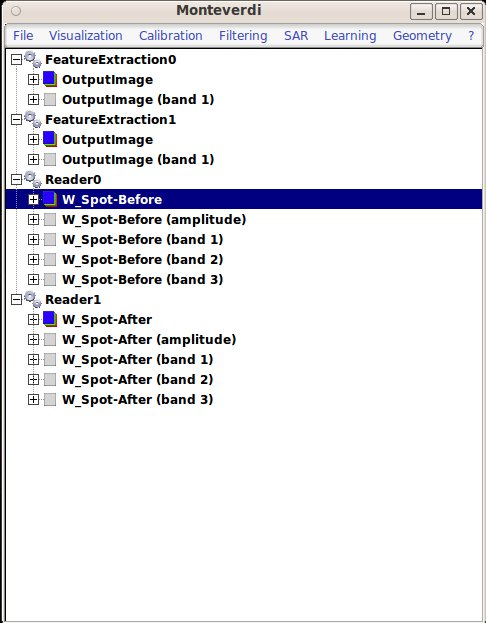
\includegraphics[width=0.9\textwidth]{monteverdi1.jpg}
\end{figure}
\end{column}
\end{columns}
\end{frame}

\begin{frame}
\frametitle{Accès facile pour les utilisateurs: Monteverdi}
\begin{figure}[]
  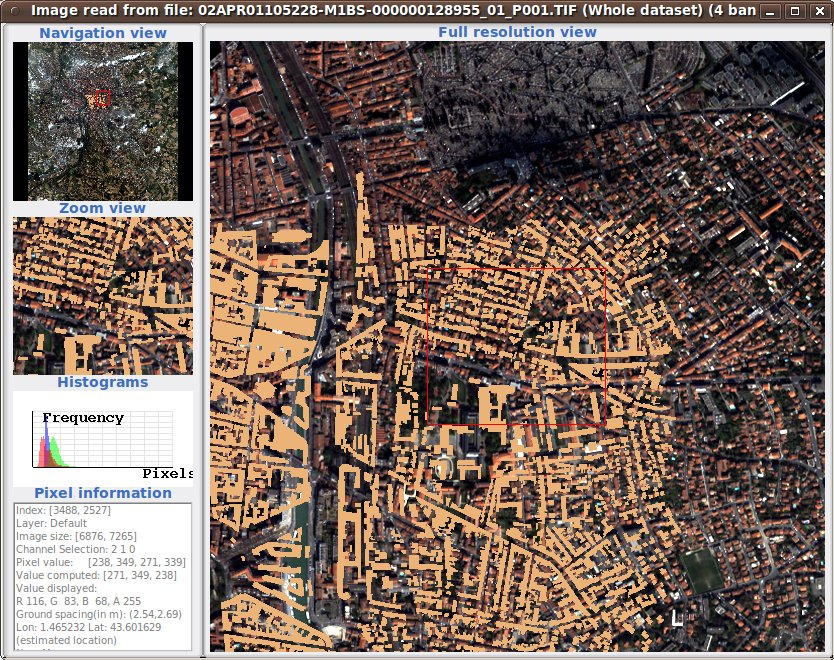
\includegraphics[width=0.8\textwidth]{monteverdi2.jpg}
\end{figure}
\end{frame}

\subsection{Bindings}
\begin{frame}
\frametitle{Bindings: accès depuis d'autres languages}
\begin{block}{Tout le monde ne programme pas en C++!}
\scriptsize
\begin{itemize}
\item Les bindings offrent un accès depuis d'autres languages deprogrammation
\item \alert{Python}: disponible
\item \alert{Java}: disponible, y compris pour d'autres languages pour
  la JVM (Clojure, Scala, etc.)
\item \alert{IDL/Envi}: coopération avec ITT VIS pour développer une
  méthode d'accès à OTB depuis IDL/ENVI (fonctionne mais difficile à
  mettre en oeuvre)
\end{itemize}
\end{block}
\end{frame}


\begin{frame}
  \frametitle{Contenu de la formation}
  \begin{enumerate}
  \item Corrections géométriques
  \item Corrections radiométriques
  \item Extraction de primitives
  \item Classification
  \item Détection de changements
  \end{enumerate}
\end{frame}
\end{document}
